% !TeX program = xelatex
\documentclass[a4paper,10pt]{article}

% ============================================================================
% សន្លឹកកិច្ចការសិស្ស ស-ខ្មៅ (Student Guided-Inquiry Worksheet - Grade 8 13.1 QUAD1)
% បរិបទ៖ ថ្នាក់រៀនគ្មានស្លាយ LCD និងមិនប្រើកន្ត្រៃកាត់ – សិស្សវាស់ និងបំពេញផ្ទាល់លើសន្លឹកកិច្ចការ ២ ទំព័រ A4
% ============================================================================
\usepackage[a4paper, left=0.90cm, right=0.90cm, top=0.75cm, bottom=0.85cm, footskip=0.45cm]{geometry}
\usepackage{amsmath, amssymb}
\usepackage{unicode-math}
\usepackage{fontspec}
\usepackage{array, colortbl}
\usepackage[table]{xcolor}
\usepackage{enumitem}
\usepackage{pifont}
\usepackage{fancyhdr}
\usepackage{lastpage}
\usepackage{tikz}
\usepackage[most]{tcolorbox}
\usetikzlibrary{calc, arrows.meta, angles, quotes, decorations.markings, positioning, babel}

\makeatletter
\let\@expl@@@mark@update@singlecol@structures@@\relax
\makeatother

\providecommand{\NGSFindFonts}{%
  \IfFileExists{C:/Windows/Fonts/cambria.ttc}{%
    \def\NGSSysPath{C:/Windows/Fonts/}%
    \def\NGSUserPath{C:/Users/KIT/AppData/Local/Microsoft/Windows/Fonts/}%
  }{%
    \IfFileExists{./fonts/KhmerOSsiemreap.ttf}{\def\NGSSysPath{./fonts/}\def\NGSUserPath{./fonts/}}{%
    \IfFileExists{../fonts/KhmerOSsiemreap.ttf}{\def\NGSSysPath{../fonts/}\def\NGSUserPath{../fonts/}}{%
    \IfFileExists{../../fonts/KhmerOSsiemreap.ttf}{\def\NGSSysPath{../../fonts/}\def\NGSUserPath{../../fonts/}}{%
    \IfFileExists{../../../fonts/KhmerOSsiemreap.ttf}{\def\NGSSysPath{../../../fonts/}\def\NGSUserPath{../../../fonts/}}{%
    \IfFileExists{../../../../fonts/KhmerOSsiemreap.ttf}{\def\NGSSysPath{../../../../fonts/}\def\NGSUserPath{../../../../fonts/}}{%
    \IfFileExists{../../../../../fonts/KhmerOSsiemreap.ttf}{\def\NGSSysPath{../../../../../fonts/}\def\NGSUserPath{../../../../../fonts/}}{%
    \IfFileExists{../../../../../../fonts/KhmerOSsiemreap.ttf}{\def\NGSSysPath{../../../../../../fonts/}\def\NGSUserPath{../../../../../../fonts/}}{%
      \def\NGSSysPath{../../../../../../../fonts/}\def\NGSUserPath{../../../../../../../fonts/}%
    }}}}}}}%
  }%
}
\NGSFindFonts

\setmathfont[Path={\NGSSysPath}, FontIndex=1, Scale=1.02]{cambria.ttc}
\defaultfontfeatures{Ligatures=TeX}

\setmainfont[
  Path={\NGSUserPath},
  Extension=.ttf,
  Script=Khmer,
  BoldFont={KhmerOSsiemreap},
  BoldFeatures={FakeBold=1.8},
  ItalicFont={KhmerOSsiemreap},
  ItalicFeatures={FakeSlant=0.25},
  BoldItalicFont={KhmerOSsiemreap},
  BoldItalicFeatures={FakeBold=1.8, FakeSlant=0.25}
]{KhmerOSsiemreap}

\newfontfamily\muol[Path={\NGSUserPath}, Extension=.ttf, Script=Khmer]{KhmerOSmuollight}
\newfontfamily\TimesEn[Path={\NGSSysPath}, Extension=.ttf, BoldFont={timesbd}, ItalicFont={timesi}, BoldItalicFont={timesbi}]{times}

\XeTeXlinebreaklocale "km"
\XeTeXlinebreakskip = 0pt plus 1pt minus 0.1pt

\definecolor{panelgray}{gray}{0.94}
\definecolor{headgray}{gray}{0.86}
\definecolor{subgray}{gray}{0.91}

\pagestyle{fancy}
\fancyhf{}
\renewcommand{\headrulewidth}{0pt}
\fancyfoot[L]{\fontsize{8pt}{10pt}\selectfont អនុវិទ្យាល័យព្រះក្រសាំង \en{|} គណិតវិទ្យា ថ្នាក់ទី៨ \en{|} មេរៀនទី១៣ (១. ប្រភេទនៃចតុកោណ)}
\fancyfoot[R]{\fontsize{8.2pt}{10pt}\selectfont ទំព័រ \en{\thepage\ / \pageref{LastPage}}}

\setlength{\parindent}{0pt}
\setlength{\parskip}{0pt}
\setlength{\tabcolsep}{4pt}

\newcommand{\en}[1]{{\TimesEn #1}}
\newcommand{\enbf}[1]{{\TimesEn\textbf{#1}}}
\newcommand{\unit}[1]{\,\text{\en{#1}}}
\newcommand{\cnum}[1]{{\fontsize{10pt}{12pt}\selectfont\ding{\numexpr171+#1\relax}}}
\newcommand{\chk}{\tikz[baseline=-0.15ex]\draw[black, line width=0.8pt] (0,0) rectangle (0.25cm,0.25cm);}
\newcommand{\ang}[1]{\ensuremath{\angle #1}}
\newcommand{\dotline}[1]{\makebox[#1]{\dotfill}}

\newcolumntype{L}[1]{>{\raggedright\arraybackslash}p{#1}}
\newcolumntype{C}[1]{>{\centering\arraybackslash}p{#1}}

\tikzset{
  tk1/.style={postaction={decorate},decoration={markings,mark=at position 0.50 with {\draw[black, line width=0.95pt](0,-0.10)--(0,0.10);}}},
  tk2/.style={postaction={decorate},decoration={markings,
    mark=at position 0.45 with {\draw[black, line width=0.95pt](0,-0.10)--(0,0.10);},
    mark=at position 0.55 with {\draw[black, line width=0.95pt](0,-0.10)--(0,0.10);}}},
  par1/.style={postaction={decorate},decoration={markings,mark=at position 0.52 with {\draw[black, line width=0.95pt](-0.07,0.08)--(0.05,0)--(-0.07,-0.08);}}},
  par2/.style={postaction={decorate},decoration={markings,
    mark=at position 0.46 with {\draw[black, line width=0.95pt](-0.07,0.08)--(0.05,0)--(-0.07,-0.08);},
    mark=at position 0.58 with {\draw[black, line width=0.95pt](-0.07,0.08)--(0.05,0)--(-0.07,-0.08);}}}
}

\newcommand{\rightbox}[4][0.20]{%
  \draw[black, line width=0.85pt]
    ($(#3)!#1!(#2)$) -- ($($(#3)!#1!(#2)$)+($(#3)!#1!(#4)$)-(#3)$) -- ($(#3)!#1!(#4)$);
}

\newcommand{\secbar}[2]{%
  \vspace{3pt}
  \noindent\colorbox{headgray}{\parbox{\dimexpr\linewidth-2\fboxsep\relax}{%
    \vspace{1.5pt}{\muol\fontsize{9.5pt}{13.5pt}\selectfont #1}\hfill{\fontsize{8.5pt}{12pt}\selectfont\textbf{#2}}\vspace{1.5pt}%
  }}\par\vspace{3pt}
}

\begin{document}
\fontsize{9.5pt}{14.5pt}\selectfont

% ============================================================================
% ទំព័រទី១៖ E1 ទស្សន៍ទាយ + E2 រុករកតារាង Van Hiele & POE រូបបង្វិល 45°
% ============================================================================
\begin{tcolorbox}[enhanced, sharp corners, colback=white, colframe=black, boxrule=1.0pt, top=4pt, bottom=4pt, left=6pt, right=6pt]
  \begin{center}
    {\muol\fontsize{10.5pt}{15pt}\selectfont សន្លឹកកិច្ចការសិស្ស — មេរៀនទី១៣៖ ចតុកោណ \enbf{(}១. ប្រភេទនៃចតុកោណ\enbf{)}}\\[2pt]
    {\footnotesize សៀវភៅសិក្សាគោលថ្នាក់ទី៨ ទំព័រ ១៦៩--១៧០ \en{|} សម្រាប់វាស់ពិនិត្យ និងបំពេញផ្ទាល់ជាដៃគូ (ដោយមិនប្រើស្លាយ \en{LCD})}
  \end{center}
  \vspace{2pt}
  \hrule height 0.5pt
  \vspace{4pt}
  ឈ្មោះសិស្សទី១៖ \dotline{3.6cm} \hspace{0.15cm} ឈ្មោះដៃគូទី២៖ \dotline{3.6cm} \hspace{0.15cm} ថ្នាក់ទី៨៖ \dotline{1.0cm} \hspace{0.15cm} ថ្ងៃទី១១/១២/២០២៦
\end{tcolorbox}

% --- E1 Engage ---
\secbar{ផ្នែកទី១ ៖ បេសកកម្មផ្ដើមមេរៀន \enbf{(E1 -- Engage)}}{៣ នាទី}
\begin{tcolorbox}[enhanced, sharp corners, colback=panelgray, colframe=black, boxrule=0.7pt, top=4pt, bottom=4pt, left=6pt, right=6pt]
  \textbf{ស្ថានភាពពិត៖} ជាងរៀបក្បឿងនៅកំពង់ស្វាយយកក្បឿងការេទំហំ $20\unit{cm}\times 20\unit{cm}$ ដដែលមកដាក់បង្វិលទ្រេត $45^\circ$ ។
  \par\vspace{2pt}
  $\bullet$ \textbf{ជាង ក ថា៖} «ពេលដាក់បង្វិល $45^\circ$ វាក្លាយជាចតុកោណស្មើ លែងជាការេ និងលែងជាចតុកោណកែងហើយ!» \par
  $\bullet$ \textbf{ជាង ខ ថា៖} «ទោះបង្វិល $45^\circ$ ក៏វានៅតែជាការេ ជាចតុកោណស្មើ និងជាចតុកោណកែងក្នុងពេលតែមួយ!» \par\vspace{3pt}
  \textbf{ការទស្សន៍ទាយដំបូងរបស់ដៃគូអ្នក (គូសធីកមុនពេលវាស់ពិសោធន៍)៖} \hspace{0.3cm} \chk\ គាំទ្រជាង ក \hspace{0.6cm} \chk\ គាំទ្រជាង ខ \hspace{0.6cm} \chk\ មិនទាន់ប្រាកដ
\end{tcolorbox}

% --- E2 Explore Act 1 ---
\secbar{ផ្នែកទី២ ៖ ពិសោធន៍វាស់ពិនិត្យ និងតារាងវិភាគលក្ខណៈ \enbf{Van Hiele (E2 -- Explore)}}{១១ នាទី}
\textbf{សកម្មភាពទី១ (៦ នាទី)៖} ប្រើ\textbf{បន្ទាត់ក្រិត} និង\textbf{ដែកកែង} វាស់ពិនិត្យរូប $Q_1$--$Q_6$ ខាងក្រោម (ខ្នាតពិតលើក្រដាស) រួចគូសសញ្ញាព្រួញស្រប (`>`, `>>`), ឆ្នូតជ្រុងស្មើ (`|`), ប្រអប់មុំកែងលើរូប និងបំពេញតារាងខាងក្រោម៖

\vspace{4pt}
\begin{center}
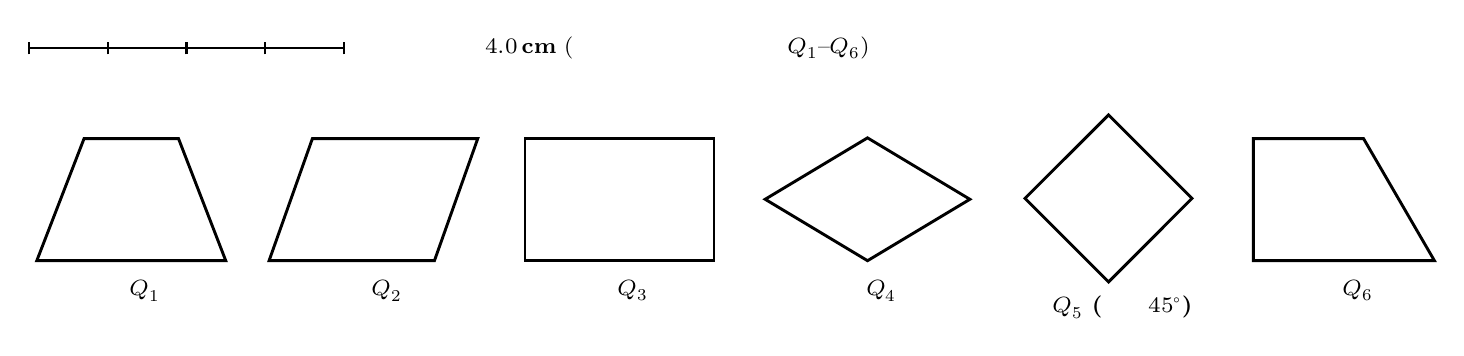
\begin{tikzpicture}[x=1cm, y=1cm, every node/.style={font=\footnotesize, text=black}]
  % ក្រិតផ្ទៀងខ្នាត 4 cm
  \draw[black, line width=0.9pt] (0,3.25) -- (4.0,3.25);
  \foreach \x in {0,1,2,3,4} { \draw[black, line width=0.8pt] (\x,3.17)--(\x,3.33); }
  \node[right=4pt] at (4.0,3.25) {\textbf{បន្ទះផ្ទៀងបន្ទាត់៖ $4.0\unit{cm}$} (ប្រើបន្ទាត់ក្រិត និងដែកកែងវាស់រូប $Q_1$--$Q_6$)};

  % Q1: ព្នាយសមបាទ
  \begin{scope}[shift={(0.1,0.55)}]
    \draw[black, line width=1.05pt] (0,0)--(2.4,0)--(1.8,1.55)--(0.6,1.55)--cycle;
    \node at (1.2,-0.38) {\textbf{រូប $Q_1$}};
  \end{scope}
  % Q2: ប្រលេឡូក្រាម
  \begin{scope}[shift={(3.05,0.55)}]
    \draw[black, line width=1.05pt] (0,0)--(2.1,0)--(2.65,1.55)--(0.55,1.55)--cycle;
    \node at (1.32,-0.38) {\textbf{រូប $Q_2$}};
  \end{scope}
  % Q3: ចតុកោណកែង
  \begin{scope}[shift={(6.30,0.55)}]
    \draw[black, line width=1.05pt] (0,0)--(2.4,0)--(2.4,1.55)--(0,1.55)--cycle;
    \node at (1.20,-0.38) {\textbf{រូប $Q_3$}};
  \end{scope}
  % Q4: ចតុកោណស្មើ
  \begin{scope}[shift={(9.35,0.55)}]
    \draw[black, line width=1.05pt] (0,0.78)--(1.30,1.56)--(2.60,0.78)--(1.30,0)--cycle;
    \node at (1.30,-0.38) {\textbf{រូប $Q_4$}};
  \end{scope}
  % Q5: ការេបង្វិល 45° (true 90 deg corners! side = 1.50 cm => half-diag = 1.061 cm)
  \begin{scope}[shift={(12.65,0.28)}]
    \draw[black, line width=1.05pt] (0,1.061)--(1.061,2.121)--(2.121,1.061)--(1.061,0)--cycle;
    \node at (1.061,-0.32) {\textbf{រូប $Q_5$ (បង្វិល $45^\circ$)}};
  \end{scope}
  % Q6: ចតុកោណព្នាយកែង
  \begin{scope}[shift={(15.55,0.55)}]
    \draw[black, line width=1.05pt] (0,0)--(2.3,0)--(1.4,1.55)--(0,1.55)--cycle;
    \node at (1.15,-0.38) {\textbf{រូប $Q_6$}};
  \end{scope}
\end{tikzpicture}
\end{center}

\vspace{3pt}
{\renewcommand{\arraystretch}{1.38}
\begin{tabular}{|C{1.25cm}|C{3.15cm}|C{3.08cm}|C{2.95cm}|C{3.25cm}|L{3.50cm}|}
  \hline
  \rowcolor{headgray}
  \textbf{រូបទី} & \textbf{ចំនួនគូជ្រុងឈមស្របគ្នា ($0, 1$ ឬ $2$ គូ)} & \textbf{ជ្រុងជាប់គ្នាប៉ុនគ្នាឬទេ? (ចាស/ទេ)} & \textbf{មានមុំកែង $90^\circ$ ឬទេ? (ចាស/ទេ)} & \textbf{ជាប្រលេឡូក្រាមឬទេ? (ចាស/ទេ)} & \multicolumn{1}{c|}{\cellcolor{headgray}\textbf{ឈ្មោះជាក់លាក់បំផុត}} \\
  \hline
  $Q_1$ & $1$ គូ & ទេ (តែជ្រុងមិនស្របស្មើ) & ទេ & ទេ & ចតុកោណព្នាយសមបាទ \\
  \hline
  $Q_2$ & \dotline{1.8cm} & \dotline{1.8cm} & \dotline{1.8cm} & \dotline{1.8cm} & \dotline{3.1cm} \\
  \hline
  $Q_3$ & \dotline{1.8cm} & \dotline{1.8cm} & \dotline{1.8cm} & \dotline{1.8cm} & \dotline{3.1cm} \\
  \hline
  $Q_4$ & \dotline{1.8cm} & \dotline{1.8cm} & \dotline{1.8cm} & \dotline{1.8cm} & \dotline{3.1cm} \\
  \hline
  $Q_5$ & \dotline{1.8cm} & \dotline{1.8cm} & \dotline{1.8cm} & \dotline{1.8cm} & \dotline{3.1cm} \\
  \hline
  $Q_6$ & \dotline{1.8cm} & \dotline{1.8cm} & \dotline{1.8cm} & \dotline{1.8cm} & \dotline{3.1cm} \\
  \hline
\end{tabular}}

\vspace{7pt}
\textbf{សកម្មភាពទី២ — ពិសោធន៍ \en{POE} បំបែកអន្ទាក់រាងគំរូ (៥ នាទី)៖}\par\vspace{3pt}
\begin{tcolorbox}[enhanced, sharp corners, colback=white, colframe=black, boxrule=0.7pt, top=5pt, bottom=5pt, left=6pt, right=6pt]
  \textbf{១. POE 2A (ពិនិត្យរូប $Q_5$ ដោយដែកកែង)៖} នៅពេលដាក់ជ្រុងកែងនៃដែកកែងលើកំពូលទាំង ៤ នៃរូប $Q_5$ តើមុំនីមួយៗស្មើប៉ុន្មានដឺក្រេ? \dotline{1.6cm} ហើយប្រវែងជ្រុងទាំង ៤ ស្មើប៉ុន្មាន $\unit{cm}$? \dotline{1.6cm} \par\vspace{2pt}
  $\Rightarrow$ ដូច្នេះ រូប $Q_5$ បំពេញនិយមន័យរបស់៖ \hspace{0.15cm} \chk\ ប្រលេឡូក្រាម \hspace{0.25cm} \chk\ ចតុកោណកែង \hspace{0.25cm} \chk\ ចតុកោណស្មើ \hspace{0.25cm} \chk\ ការេ ។ \par\vspace{4pt}
  \textbf{២. POE 2B (ប្រយ័ត្នទិសដៅព្រួញ!)៖} ចូរគូសធីក \textbf{ពិត} ឬ \textbf{មិនពិត} និងបំពេញហេតុផល៖ \par\vspace{2pt}
  $\bullet$ (ក) «គ្រប់ការេទាំងអស់សុទ្ធតែជាចតុកោណកែង»៖ \hspace{0.2cm} \chk\ ពិត \hspace{0.2cm} \chk\ មិនពិត ព្រោះការេជាប្រលេឡូក្រាមដែលមានមុំ \dotline{1.8cm} ។ \par\vspace{2pt}
  $\bullet$ (ខ) «គ្រប់ចតុកោណកែងទាំងអស់សុទ្ធតែជាការេ»៖ \hspace{0.2cm} \chk\ ពិត \hspace{0.2cm} \chk\ មិនពិត ព្រោះរូប $Q_3$ មានជ្រុងជាប់ \dotline{2.5cm} គ្នា ។
\end{tcolorbox}

% ============================================================================
% ទំព័រទី២៖ E3 សង្ខេបនិយមន័យ & គំនូសតាង + E4 លំហាត់គំរូ + E5 ប្រតិបត្តិ & Exit + កិច្ចការផ្ទះ
% ============================================================================
\newpage

\secbar{ផ្នែកទី៣ ៖ សង្ខេបនិយមន័យ ធនាគារហេតុផល \cnum{1}\enbf{--}\cnum{5} និងគំនូសតាងឋានានុក្រម \enbf{(E3 -- Explain)}}{៦ នាទី}
\begin{tabular}{@{}L{9.45cm}|L{9.35cm}@{}}
  \textbf{ធនាគារនិយមន័យគោល (សៀវភៅគោល ទំ.១៦៩--១៧០)៖}\par\vspace{3pt}
  \cnum{1}\ \textbf{ចតុកោណព្នាយ៖} ចតុកោណមានជ្រុងពីរ \dotline{1.8cm} គ្នា ($AB\parallel DC$) ។\par
  \hspace*{0.45cm}– ជ្រុងមិនស្របស្មើគ្នា $\to$ \textbf{ព្នាយសមបាទ}; មុំកែងមួយ $\to$ \textbf{ព្នាយកែង} ។\par\vspace{2pt}
  \cnum{2}\ \textbf{ប្រលេឡូក្រាម៖} ចតុកោណមានជ្រុងឈម \dotline{1.8cm} គ្នាពីរៗ ។\par\vspace{2pt}
  \cnum{3}\ \textbf{ចតុកោណកែង៖} ប្រលេឡូក្រាមដែលមាន \dotline{2.2cm} មួយ ។\par\vspace{2pt}
  \cnum{4}\ \textbf{ចតុកោណស្មើ៖} ប្រលេឡូក្រាមដែលមានជ្រុងជាប់គ្នា \dotline{1.8cm} គ្នា ។\par\vspace{2pt}
  \cnum{5}\ \textbf{ការេ៖} ប្រលេឡូក្រាមមានជ្រុងពីរជាប់គ្នាស្មើគ្នា និងមានមុំកែងមួយ ។
  &
  \textbf{បំពេញឈ្មោះក្នុងគំនូសតាងទំនាក់ទំនង (ទំ.១៧០)៖}\par\vspace{4pt}
  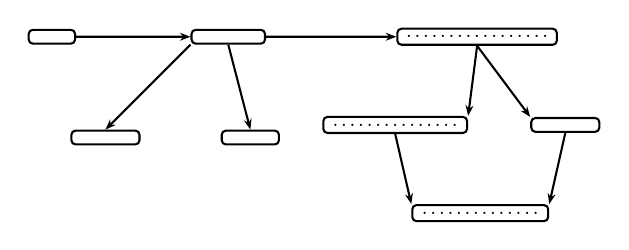
\begin{tikzpicture}[scale=0.80, every node/.style={font=\scriptsize, text=black},
    bx/.style={draw=black, line width=0.75pt, rounded corners=1.5pt, fill=white, inner sep=2.5pt, align=center}]
    \node[bx] (q) at (0,2.25) {ចតុកោណ};
    \node[bx] (t) at (2.80,2.25) {ចតុកោណព្នាយ};
    \node[bx] (p) at (6.75,2.25) {\dotline{1.85cm}};
    \node[bx] (it) at (0.85,0.65) {ព្នាយសមបាទ};
    \node[bx] (rt) at (3.15,0.65) {ព្នាយកែង};
    \node[bx] (rc) at (5.45,0.85) {\dotline{1.65cm}};
    \node[bx] (rh) at (8.15,0.85) {ចតុកោណស្មើ};
    \node[bx] (sq) at (6.80,-0.55) {\dotline{1.55cm}};
    \draw[-{Stealth[length=3.8pt]}, line width=0.75pt] (q)--(t);
    \draw[-{Stealth[length=3.8pt]}, line width=0.75pt] (t)--(p);
    \draw[-{Stealth[length=3.8pt]}, line width=0.75pt] (t.south west)--(it.north);
    \draw[-{Stealth[length=3.8pt]}, line width=0.75pt] (t.south)--(rt.north);
    \draw[-{Stealth[length=3.8pt]}, line width=0.75pt] (p.south)--(rc.north east);
    \draw[-{Stealth[length=3.8pt]}, line width=0.75pt] (p.south)--(rh.north west);
    \draw[-{Stealth[length=3.8pt]}, line width=0.75pt] (rc.south)--(sq.north west);
    \draw[-{Stealth[length=3.8pt]}, line width=0.75pt] (rh.south)--(sq.north east);
  \end{tikzpicture}
\end{tabular}

% --- E4 Elaborate ---
\secbar{ផ្នែកទី៤ ៖ លំហាត់គំរូអនុវត្ត \enbf{[tracing]} និងធនាគារហេតុផល \cnum{1}\enbf{--}\cnum{5} \enbf{(E4 -- Elaborate)}}{១០ នាទី}
ចូរគូសសញ្ញាសម្គាល់លើរូប (ក)--(ឃ) រួចបំពេញឈ្មោះចតុកោណជាក់លាក់បំផុត និងលេខហេតុផល \cnum{1}--\cnum{5}៖

\vspace{3pt}
{\renewcommand{\arraystretch}{1.35}
\begin{tabular}{|C{4.45cm}|C{4.45cm}|C{4.45cm}|C{4.45cm}|}
  \hline
  \rowcolor{subgray}
  \textbf{(ក) $AB\parallel DC, AD\parallel BC, \ang{B}=90^\circ$} &
  \textbf{(ខ) មានតែ $MN\parallel PO$ និង $MP=NO$} &
  \textbf{(គ) ប្រលេឡូក្រាម $EF=EH=4\unit{cm}$} &
  \textbf{(ឃ) ចតុកោណកែងមាន $RS=ST$} \\
  \hline
  \vspace{2pt}
  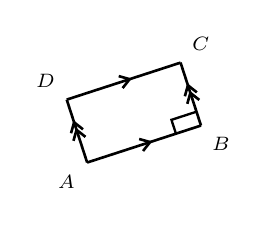
\begin{tikzpicture}[scale=0.80, every node/.style={font=\scriptsize}]
    \begin{scope}[rotate=18]
      \draw[line width=0.95pt, par1] (0,1.05)--(1.9,1.05);
      \draw[line width=0.95pt, par1] (0,0)--(1.9,0);
      \draw[line width=0.95pt, par2] (0,0)--(0,1.05);
      \draw[line width=0.95pt, par2] (1.9,0)--(1.9,1.05);
      \rightbox[0.22]{0,0}{1.9,0}{1.9,1.05}
      \node[below left=1pt] at (0,0) {$A$}; \node[below right=1pt] at (1.9,0) {$B$};
      \node[above right=1pt] at (1.9,1.05) {$C$}; \node[above left=1pt] at (0,1.05) {$D$};
    \end{scope}
  \end{tikzpicture}
  &
  \vspace{2pt}
  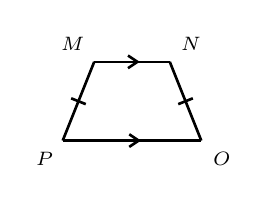
\begin{tikzpicture}[scale=0.80, every node/.style={font=\scriptsize}]
    \draw[line width=0.95pt, par1] (0.5,1.25)--(1.7,1.25);
    \draw[line width=0.95pt, par1] (0,0)--(2.2,0);
    \draw[line width=0.95pt, tk1] (0,0)--(0.5,1.25);
    \draw[line width=0.95pt, tk1] (2.2,0)--(1.7,1.25);
    \node[below left=1pt] at (0,0) {$P$}; \node[below right=1pt] at (2.2,0) {$O$};
    \node[above right=1pt] at (1.7,1.25) {$N$}; \node[above left=1pt] at (0.5,1.25) {$M$};
  \end{tikzpicture}
  &
  \vspace{2pt}
  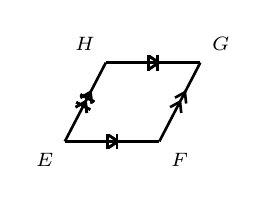
\begin{tikzpicture}[scale=0.80, every node/.style={font=\scriptsize}]
    \draw[line width=0.95pt, par1, tk2] (0.65,1.25)--(2.15,1.25);
    \draw[line width=0.95pt, par1, tk2] (0,0)--(1.50,0);
    \draw[line width=0.95pt, par2, tk2] (0,0)--(0.65,1.25);
    \draw[line width=0.95pt, par2] (1.50,0)--(2.15,1.25);
    \node[below left=1pt] at (0,0) {$E$}; \node[below right=1pt] at (1.5,0) {$F$};
    \node[above right=1pt] at (2.15,1.25) {$G$}; \node[above left=1pt] at (0.65,1.25) {$H$};
  \end{tikzpicture}
  &
  \vspace{2pt}
  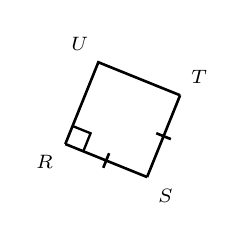
\begin{tikzpicture}[scale=0.80, every node/.style={font=\scriptsize}]
    \begin{scope}[rotate=-22]
      \draw[line width=0.95pt, tk1] (0,0)--(1.4,0);
      \draw[line width=0.95pt, tk1] (1.4,0)--(1.4,1.4);
      \draw[line width=0.95pt] (1.4,1.4)--(0,1.4)--(0,0);
      \rightbox[0.22]{1.4,0}{0,0}{0,1.4}
      \node[below left=1pt] at (0,0) {$R$}; \node[below right=1pt] at (1.4,0) {$S$};
      \node[above right=1pt] at (1.4,1.4) {$T$}; \node[above left=1pt] at (0,1.4) {$U$};
    \end{scope}
  \end{tikzpicture} \\
  \hline
  ប្រភេទ៖ \dotline{2.8cm}\par ហេតុផលលេខ៖ \dotline{1.4cm} &
  ប្រភេទ៖ \dotline{2.8cm}\par ហេតុផលលេខ៖ \dotline{1.4cm} &
  ប្រភេទ៖ \dotline{2.8cm}\par ហេតុផលលេខ៖ \dotline{1.4cm} &
  ប្រភេទ៖ \dotline{2.8cm}\par ហេតុផលលេខ៖ \dotline{1.4cm} \\
  \hline
\end{tabular}}

% --- E5 Evaluate ---
\secbar{ផ្នែកទី៥ ៖ លំហាត់ប្រតិបត្តិ ផ្ទៀងផ្ទាត់ជាដៃគូ និង \enbf{Exit Check (E5 -- Evaluate)}}{១០ នាទី}
\textbf{ក. លំហាត់ប្រតិបត្តិ៖} គូសធីក \textbf{ពិត} ឬ \textbf{មិនពិត} រួចសរសេរលេខហេតុផល និងគូសរូបឧទាហរណ៍ផ្ទុយសម្រាប់សំណើទី២៖
\par\vspace{3pt}
\begin{tabular}{@{}L{12.15cm} C{6.65cm}@{}}
  ១. «គ្រប់ចតុកោណស្មើទាំងអស់សុទ្ធតែជាប្រលេឡូក្រាម»៖ \hspace{0.1cm} \chk\ ពិត \hspace{0.1cm} \chk\ មិនពិត\par
  \hspace*{0.4cm}ហេតុផល៖ \dotline{9.2cm}\par\vspace{4pt}
  ២. «គ្រប់ប្រលេឡូក្រាមទាំងអស់សុទ្ធតែជាចតុកោណកែង»៖ \hspace{0.1cm} \chk\ ពិត \hspace{0.1cm} \chk\ មិនពិត\par
  \hspace*{0.4cm}ពន្យល់៖ \dotline{9.5cm}\par\vspace{4pt}
  ៣. «គ្រប់ការេទាំងអស់ជាចតុកោណស្មើផង និងចតុកោណកែងផង»៖ \chk\ ពិត \hspace{0.1cm} \chk\ មិនពិត\par
  \hspace*{0.4cm}ហេតុផល៖ \dotline{9.2cm}\par\vspace{4pt}
  ៤. \textbf{បិទបញ្ហាជាងក្បឿង E1៖} សម្ដីរបស់ជាង \dotline{1.2cm} ត្រឹមត្រូវ ព្រោះ \dotline{6.8cm}
  &
  \begin{tikzpicture}[x=1cm,y=1cm, baseline={(0,2.85)}]
    \draw[black, line width=0.8pt, dashed] (0,0) rectangle (6.45,3.25);
    \node[font=\footnotesize] at (3.22,2.92) {\textbf{ប្រអប់គូសរូបឧទាហរណ៍ផ្ទុយ (សំណើទី២)}};
    \node[font=\scriptsize] at (3.22,0.28) {(គូសប្រលេឡូក្រាមដែលមិនមែនជាចតុកោណកែង)};
  \end{tikzpicture}
\end{tabular}

\vspace{5pt}
\begin{tcolorbox}[enhanced, sharp corners, colback=panelgray, colframe=black, boxrule=0.8pt, top=4pt, bottom=4pt, left=6pt, right=6pt]
  \textbf{ខ. សំណួរត្រួតពិនិត្យរហ័ស (\en{Exit Check} — គូសរង្វង់ចម្លើយត្រឹមត្រូវតែ ១)៖}\par
  បើចតុកោណ $ABCD$ មាន $AB\parallel DC$, $AD\parallel BC$, $AB=BC=5\unit{cm}$ ប៉ុន្តែមុំ $\ang{A}=65^\circ$ តើឈ្មោះជាក់លាក់បំផុតរបស់វាគឺអ្វី?\par\vspace{2pt}
  \hspace*{0.4cm}\textbf{A.} ចតុកោណកែង \hspace{1.6cm} \textbf{B.} ការេ \hspace{1.8cm} \textbf{C.} ចតុកោណស្មើ \hspace{1.6cm} \textbf{D.} ចតុកោណព្នាយកែង
\end{tcolorbox}

% --- Step 5 Homework ---
\secbar{ផ្នែកទី៦ ៖ កិច្ចការផ្ទះ និងបណ្ដាំផ្ញើ \enbf{(}សៀវភៅគោល ទំ.១៧០ និងទំ.១៨៥\enbf{)}}{ធ្វើក្នុងសៀវភៅកិច្ចការផ្ទះ}
$\bullet$ \textbf{លំហាត់ទី១ (លំហាត់ទី៦ ក ទំព័រ ១៨៥)៖} សង់ប្រលេឡូក្រាម $ABCD$ ដោយស្គាល់ $\ang{A}=60^\circ$, $AB=6\unit{cm}$ និង $AD=4\unit{cm}$ ។ តើ $ABCD$ អាចជាចតុកោណកែង ឬចតុកោណស្មើបានដែរឬទេ? ចូរពន្យល់ដោយផ្អែកលើនិយមន័យ \cnum{3} និង \cnum{4} ។ \par\vspace{2pt}
$\bullet$ \textbf{លំហាត់ទី២៖} គូសគំនូសតាងទំនាក់ទំនងនៃប្រភេទចតុកោណ (ទំ.១៧០) ចូលសៀវភៅសរសេរ និងអានជាមុន \textbf{២.១ លក្ខណៈប្រលេឡូក្រាម} (ទំ.១៧០--១៧១) ។

\end{document}
